\begin{frame}{Autonomie}
	\alt<1>{\begin{itemize}
		\item{Vereinigung von \textcolor{vertexLightGrey}{Dynamik} und Unabhängigkeit}
			\begin{itemize}
				\item{\textcolor{vertexLightGrey}{Informationsverarbeitung}}
			\end{itemize}
		\item{Maß für Dynamik}
	\end{itemize}
	\begin{beamerboxesrounded}{Energie-Kohärenz}
		\begin{empheq}{equation*}
			\delta H = \frac{1}{\sqrt{2}} \norm{\dot{\rho}} = \sqrt{\Tr\sbr{H^{2}\rho^{2} - H\rho H\rho}}
		\end{empheq}
		\vspace{-0.5cm}
	\end{beamerboxesrounded}}{}
	\alt<2>{\begin{itemize}
		\item{Unterschiedliche Grade an Dynamik:}
	\end{itemize}
	\begin{columns}
		\begin{column}{0.3\textwidth}
			\centering
			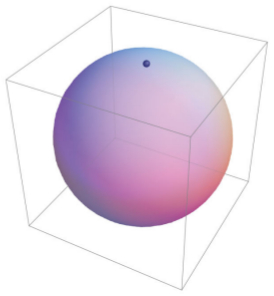
\includegraphics[scale=.3]{graphics/autonomy_static.jpg}
		\end{column}
		\begin{column}{0.3\textwidth}
			\centering
			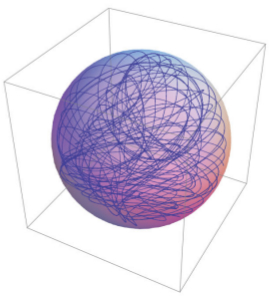
\includegraphics[scale=.3]{graphics/autonomy_chaotic.jpg}
		\end{column}
		\begin{column}{0.3\textwidth}
			\centering
			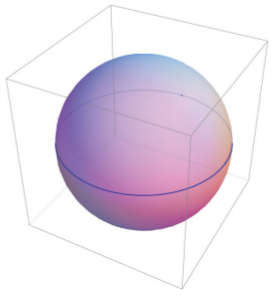
\includegraphics[scale=.3]{graphics/autonomy_simple.jpg}
		\end{column}
	\end{columns}
	\begin{itemize}
		\item{Reduktion der maximalen Energie-Kohärenz um wenige Prozent}
			\begin{itemize}
				\item{Komplexe, chaotische Dynamik möglich}
			\end{itemize}
	\end{itemize}}{}
\end{frame}